\subsection{Collinear Solutions \texorpdfstring{($y = 0$)}{}}

From Equation~(\refeq{eq:roots}), we have
\begin{equation}
    \cm x \cw - \ddfrac{\left(1 - \cred \mu \cw \right) \left(\cm x \cw + \cred \mu \cw\right)}{\cc r_1 \cw ^3} - \ddfrac{\cred \mu \cw \left(\cm x \cw - 1 + \cred\mu\cw\right)}{\cg r_2 \cw ^3} = 0
    \label{eq:rootsX}
\end{equation}

Recall that
\begin{equation*}
    \cc r_1 \cw ^2 = \left(\cm x \cw + \cred\mu\cw\right)^2 + \cm y \cw ^2 \qquad \cg r_2 \cw ^2 = \left(\cm x \cw - 1 + \cred\mu\cw\right)^2 + \cm y \cw ^2
\end{equation*}

By setting $y = 0$, Equation~\eqref{eq:rootsX} becomes
\begin{equation}
    \cm x \cw \, \tikzmarknode{A}{-} \, \ddfrac{\left(1 - \cred \mu \cw \right) \left(\cm x \cw + \cred \mu \cw\right)}{\left(\sqrt{\left(\cm x \cw + \cred\mu\cw\right)^2}\right)^3} \, \tikzmarknode{B}{-} \, \ddfrac{\cred \mu \cw \left(\cm x \cw - 1 + \cred\mu\cw\right)}{\left(\sqrt{\left(\cm x \cw - 1 + \cred\mu\cw\right)^2}\right)^3} = 0  \\
    \label{eq:eq6}
    \begin{tikzpicture}[overlay, remember picture]
        % Calculate points for the start and end of the blue arrow
        \coordinate (startBlue) at ($(A)+(-0.2, -0.9)$);
        \coordinate (endBlue) at ($(startBlue)+(0.2, 0.75)$);

        % Calculate points for the start and end of the green arrow
        \coordinate (startGreen) at ($(B)+(-0.2, -0.9)$);
        \coordinate (endGreen) at ($(startGreen)+(0.2, 0.75)$);

        % Draw the blue arrow
        \draw[blue,-latex, thick] (startBlue) -- (endBlue);

        % Draw the green arrow
        \draw[green,-latex, thick] (startGreen) -- (endGreen);
    \end{tikzpicture}
\end{equation}

In Equation~\eqref{eq:eq6}, there may be a temptation to cancel terms prematurely but this could potentially eliminate valid solutions. Let's consider four scenarios that correspond to the second and third terms in \eqref{eq:eq6} being either positive or negative before further simplifying the equation.

\vspace{\baselineskip}

\underline{Scenario 1}: \quad $\cm x \cw + \cred \mu \cw > 0$, \quad $\cm x \cw - 1 + \cred \mu \cw < 0$ \quad $\longrightarrow$ \quad $\cm x \cw > - \cred \mu \cw$, \quad $\cm x \cw < 1 - \cred \mu \cw$

\begin{center}
    \vspace{7pt}
    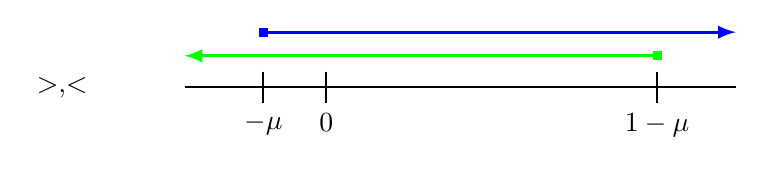
\begin{tikzpicture}
        % Draw the horizontal line
        \draw[thick] (-3,0) -- (4,0);

        % Draw the ticks and labels
        \draw[thick] (-2,0.2) -- (-2,-0.2) node[below] {$- \cred \mu$};
        \draw[thick] (-1.2,0.2) -- (-1.2,-0.2) node[below] {0};
        \draw[thick] (3,0.2) -- (3,-0.2) node[below] {$1-\cred \mu$};

        % Draw the blue arrow with square
        \filldraw[blue] (-1.95,0.65) rectangle (-2.05,0.75); % Make square thinner
        \draw[blue, very thick, -latex] (-2,0.7) -- (4,0.7); % Start slightly above the line

        % Draw the green arrow with square
        \filldraw[green] (2.95,0.35) rectangle (3.05,0.45); % Make square thinner
        \draw[green, very thick, -latex] (3,0.4) -- (-3,0.4); % Start slightly above the line
        % Add a node for text at a certain position
        \node[anchor=west] at (-5,0) {$\cb >$,$\cg <$};
    \end{tikzpicture}
\end{center}

This corresponds to a solution that lies between the two bodies.

\vspace{\baselineskip}

\underline{Scenario 2}: \quad $\cm x \cw + \cred \mu \cw > 0$, \quad $\cm x \cw - 1 + \cred \mu \cw > 0$ \quad $\longrightarrow$ \quad $\cm x \cw > - \cred \mu \cw$, \quad $\cm x \cw > 1 - \cred \mu \cw$

\begin{center}
    \vspace{7pt}
    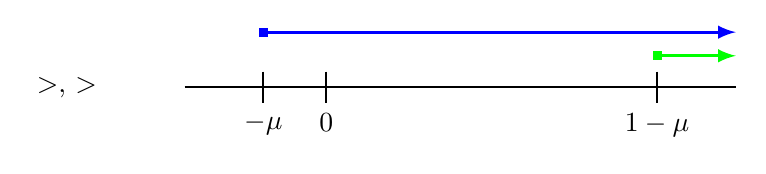
\begin{tikzpicture}
        % Draw the horizontal line
        \draw[thick] (-3,0) -- (4,0);

        % Draw the ticks and labels
        \draw[thick] (-2,0.2) -- (-2,-0.2) node[below] {$- \cred \mu$};
        \draw[thick] (-1.2,0.2) -- (-1.2,-0.2) node[below] {0};
        \draw[thick] (3,0.2) -- (3,-0.2) node[below] {$1-\cred \mu$};

        % Draw the blue arrow with square
        \filldraw[blue] (-1.95,0.65) rectangle (-2.05,0.75); % Make square thinner
        \draw[blue, very thick, -latex] (-2,0.7) -- (4,0.7); % Start slightly above the line

        % Draw the green arrow with square
        \filldraw[green] (2.95,0.35) rectangle (3.05,0.45); % Make square thinner
        \draw[green, very thick, -latex] (3,0.4) -- (4,0.4); % Start slightly above the line
        % Add a node for text at a certain position
        \node[anchor=west] at (-5,0) {$\cb >$, $\cg >$};
    \end{tikzpicture}
\end{center}

From above, we can see that both inequalities are true when $\cm x \cw > 1 - \cred \mu \cw$. We don't know what this value is yet, but we know that it must lie on the right side of the smaller body (Moon).

\vspace{\baselineskip}

\underline{Scenario 3}: \quad $\cm x \cw + \cred \mu \cw < 0$, \quad $\cm x \cw - 1 + \cred \mu \cw > 0$ \quad $\longrightarrow$ \quad $\cm x \cw < - \cred \mu \cw$, \quad $\cm x \cw > 1 - \cred \mu \cw$

\begin{center}
    \vspace{7pt}
    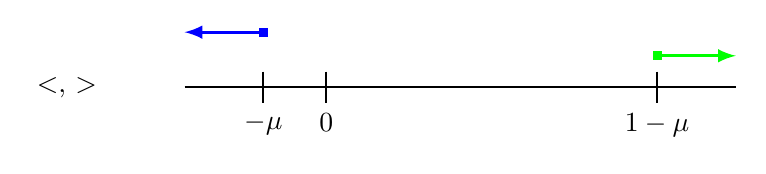
\begin{tikzpicture}
        % Draw the horizontal line
        \draw[thick] (-3,0) -- (4,0);

        % Draw the ticks and labels
        \draw[thick] (-2,0.2) -- (-2,-0.2) node[below] {$- \cred \mu$};
        \draw[thick] (-1.2,0.2) -- (-1.2,-0.2) node[below] {0};
        \draw[thick] (3,0.2) -- (3,-0.2) node[below] {$1-\cred \mu$};

        % Draw the blue arrow with square
        \filldraw[blue] (-1.95,0.65) rectangle (-2.05,0.75); % Make square thinner
        \draw[blue, very thick, -latex] (-2,0.7) -- (-3,0.7); % Start slightly above the line

        % Draw the green arrow with square
        \filldraw[green] (2.95,0.35) rectangle (3.05,0.45); % Make square thinner
        \draw[green, very thick, -latex] (3,0.4) -- (4,0.4); % Start slightly above the line

        % Add a node for text at a certain position
        \node[anchor=west] at (-5,0) {$\cb <$, $\cg >$};
    \end{tikzpicture}
\end{center}

This leads to an \cy invalid solution \cw since these conditions do not overlap (there are no values of $\cm x \cw$ that are both less than $\cred \mu$ and greater than $1 - \cred \mu$).

\vspace{\baselineskip}

\underline{Scenario 4}: \quad $\cm x \cw + \cred \mu \cw < 0$, \quad $\cm x \cw - 1 + \cred \mu \cw < 0$ \quad $\longrightarrow$ \quad $\cm x \cw < - \cred \mu \cw$, \quad $\cm x \cw < 1 - \cred \mu \cw$

\begin{center}
    \vspace{7pt}
    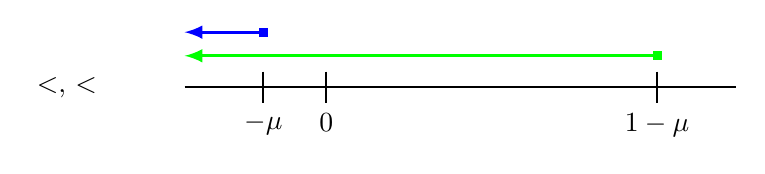
\begin{tikzpicture}
        % Draw the horizontal line
        \draw[thick] (-3,0) -- (4,0) ;

        % Draw the ticks and labels
        \draw[thick] (-2,0.2) -- (-2,-0.2) node[below] {$- \cred \mu$};
        \draw[thick] (-1.2,0.2) -- (-1.2,-0.2) node[below] {0};
        \draw[thick] (3,0.2) -- (3,-0.2) node[below] {$1-\cred \mu$};

        % Draw the blue arrow with square
        \filldraw[blue] (-1.95,0.65) rectangle (-2.05,0.75); % Make square thinner
        \draw[blue, very thick, -latex] (-2,0.7) -- (-3,0.7); % Start slightly above the line

        % Draw the green arrow with square
        \filldraw[green] (2.95,0.35) rectangle (3.05,0.45); % Make square thinner
        \draw[green, very thick, -latex] (3,0.4) -- (-3,0.4); % Start slightly above the line

        % Add a node for text at a certain position
        \node[anchor=west] at (-5,0) {$\cb <$, $\cg <$};

    \end{tikzpicture}
\end{center}

This corresponds to a solution that lies to the left of the larger body (Earth).

\pagebreak

Now, we can simplify Equation~\eqref{eq:eq6} corresponding to each scenario we looked at above:

\begin{center}
    \noindent\fcolorbox{red}{black}{
        $ f_1(\cm x \cw) =  \cm x \cw - \ddfrac{1 - \cred \mu \cw}{\left(\cm x \cw + \cred\mu\cw\right)^2} + \ddfrac{\cred \mu \cw}{\left(\cm x \cw - 1 + \cred\mu\cw\right)^2} = 0 $
    } \\ \vspace{5pt}
    \noindent\fcolorbox{green}{black}{
        $ f_2(\cm x \cw) = \cm x \cw - \ddfrac{1 - \cred \mu \cw}{\left(\cm x \cw + \cred\mu\cw\right)^2} - \ddfrac{\cred \mu \cw}{\left(\cm x \cw - 1 + \cred\mu\cw\right)^2} = 0 $
    } \\ \vspace{5pt}
    \noindent\fcolorbox{yellow}{black}{
        $ f_3(\cm x \cw) = \cm x \cw + \ddfrac{1 - \cred \mu \cw}{\left(\cm x \cw + \cred\mu\cw\right)^2} - \ddfrac{\cred \mu \cw}{\left(\cm x \cw - 1 + \cred\mu\cw\right)^2} = 0 $
    } \\ \vspace{5pt}
    \noindent\fcolorbox{blue}{black}{
        $ f_4(\cm x \cw) = \cm x \cw + \ddfrac{1 - \cred \mu \cw}{\left(\cm x \cw + \cred\mu\cw\right)^2} + \ddfrac{\cred \mu \cw}{\left(\cm x \cw - 1 + \cred\mu\cw\right)^2} = 0 $
    } \\ \vspace{5pt}
\end{center}

Having completed that process, the simplified equations above can be plotted, with careful attention to the positive and negative signs, to confirm the expected solutions. 

\begin{figure}[h]
    \centering
    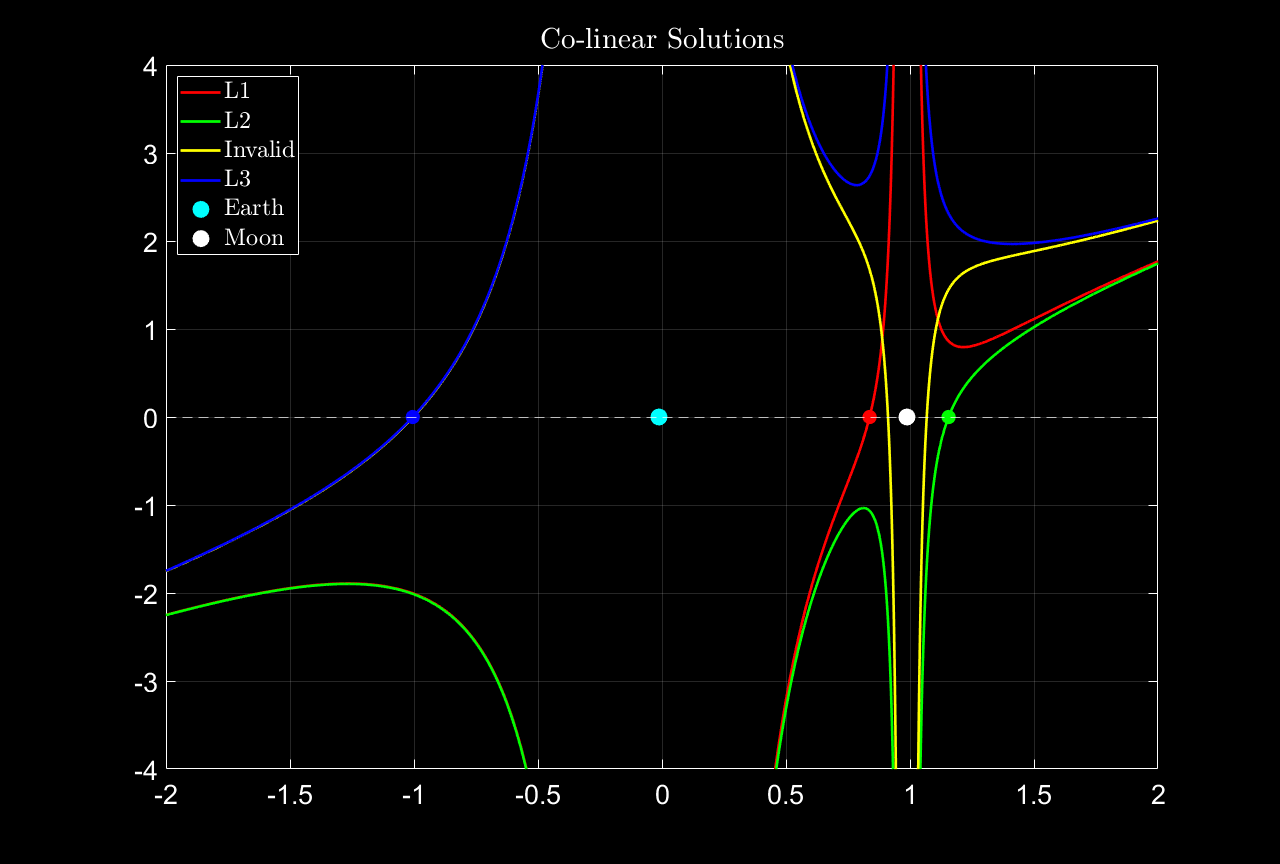
\includegraphics[width=\textwidth]{fig/lagrange123.png}
    \caption{Graphical Representation of the Collinear Solutions for the Lagrange points}
    \label{fig:lagrange_points}
\end{figure}

It is noted that these collinear solutions are determined using a numerical root-solving method (secant method) that utilizes finite differences for the estimation of derivatives and iteratively converges on the solutions. These solutions correspond to the x-coordinates of the Lagrange points ($L_1$--$L_3$), and the Earth and Moon are marked to indicate their relative positions in this configuration.

\vspace{\baselineskip}

\pagebreak

The coordinates of $L_1$, $L_2$, and $L_3$ are summarized below:

\begin{table}[h]
    \centering
    \caption{\cw Collinear Lagrange Points for Earth-Moon System}
    \begin{tabular}{ccc} \toprule
        {Lagrange Point} & {$x$} & {$y$}   \\ \midrule
        $L_1$ \cw  &  0.837023544523  & 0   \\
        $L_2$ \cw  &  1.155597402589  & 0   \\
        $L_3$ \cw  & -1.005053470159  & 0   \\  \bottomrule
    \end{tabular}
    \label{tab:table3}
\end{table}